\documentclass[11pt]{article}
\usepackage[a4paper, total={7in, 8in}]{geometry}

\usepackage[utf8]{inputenc}
\usepackage[french]{babel}
\usepackage{graphicx}
\usepackage{url}
\usepackage[colorlinks = true,urlcolor = blue]{hyperref}
\usepackage[T1]{fontenc}
\usepackage[acronym,nomain]{glossaries}
\usepackage{hyperref}
\frenchbsetup{og=«,fg=»}  
\hypersetup
{
    allcolors = black
}

\title{Une traversé de Paris pont à pont}
\author{Les membres des Mardis numériques du \today}

\begin{document}
\maketitle

\begin{abstract}
    Une expérience de récit collaboratif du paysage urbain entre les ponts de Tolbiac et Mirabeau.
\end{abstract}

\section*{Du pont de Tolbiac au pont de Bercy}

%Copiez la totalité du contenue entre \begin{figure} et \end{figure} pour insérer une autre figure, et changez simplement \includegraphics[width=12cm]{images/NOM_DU_FICHIER}
\begin{figure}[h]
\centering
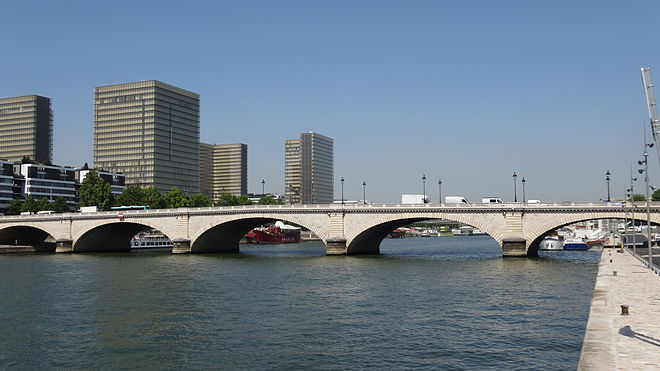
\includegraphics[width=15cm]{images/pont_de_tolbiac}
\caption{Le pont de Tolbiac vu du port de Bercy}
\end{figure}


\section*{Du pont de Bercy au pont Charles de Gaulle}

\section*{Du pont Charles de Gaulle au pont d'Austerlitz}

\section*{Du pont d'Austerlitz au pont de Sully}

\section*{Du pont de Sully au pont Marie}

\section*{Du pont Marie au point Louis Philippe}

\section*{Du point Louis Philippe au pont d'Arcole}

\section*{Du pont d'Arcole au pont au Change}

\section*{Du pont au Change au pont Neuf}

\section*{Du pont Neuf au pont du Carrousel}

\section*{Du pont du Carrousel au pont de la Concorde}

\section*{Du pont de la Concorde au pont des invalides}

\section*{Du pont des invalides au pont de Bir-Hakeim}

\section*{Du pont de Bir-Hakeim au pont Mirabeau}


\end{document}